\appendix

\chapter{Model predictions}

\begin{figure}[!htb]
    \centering
    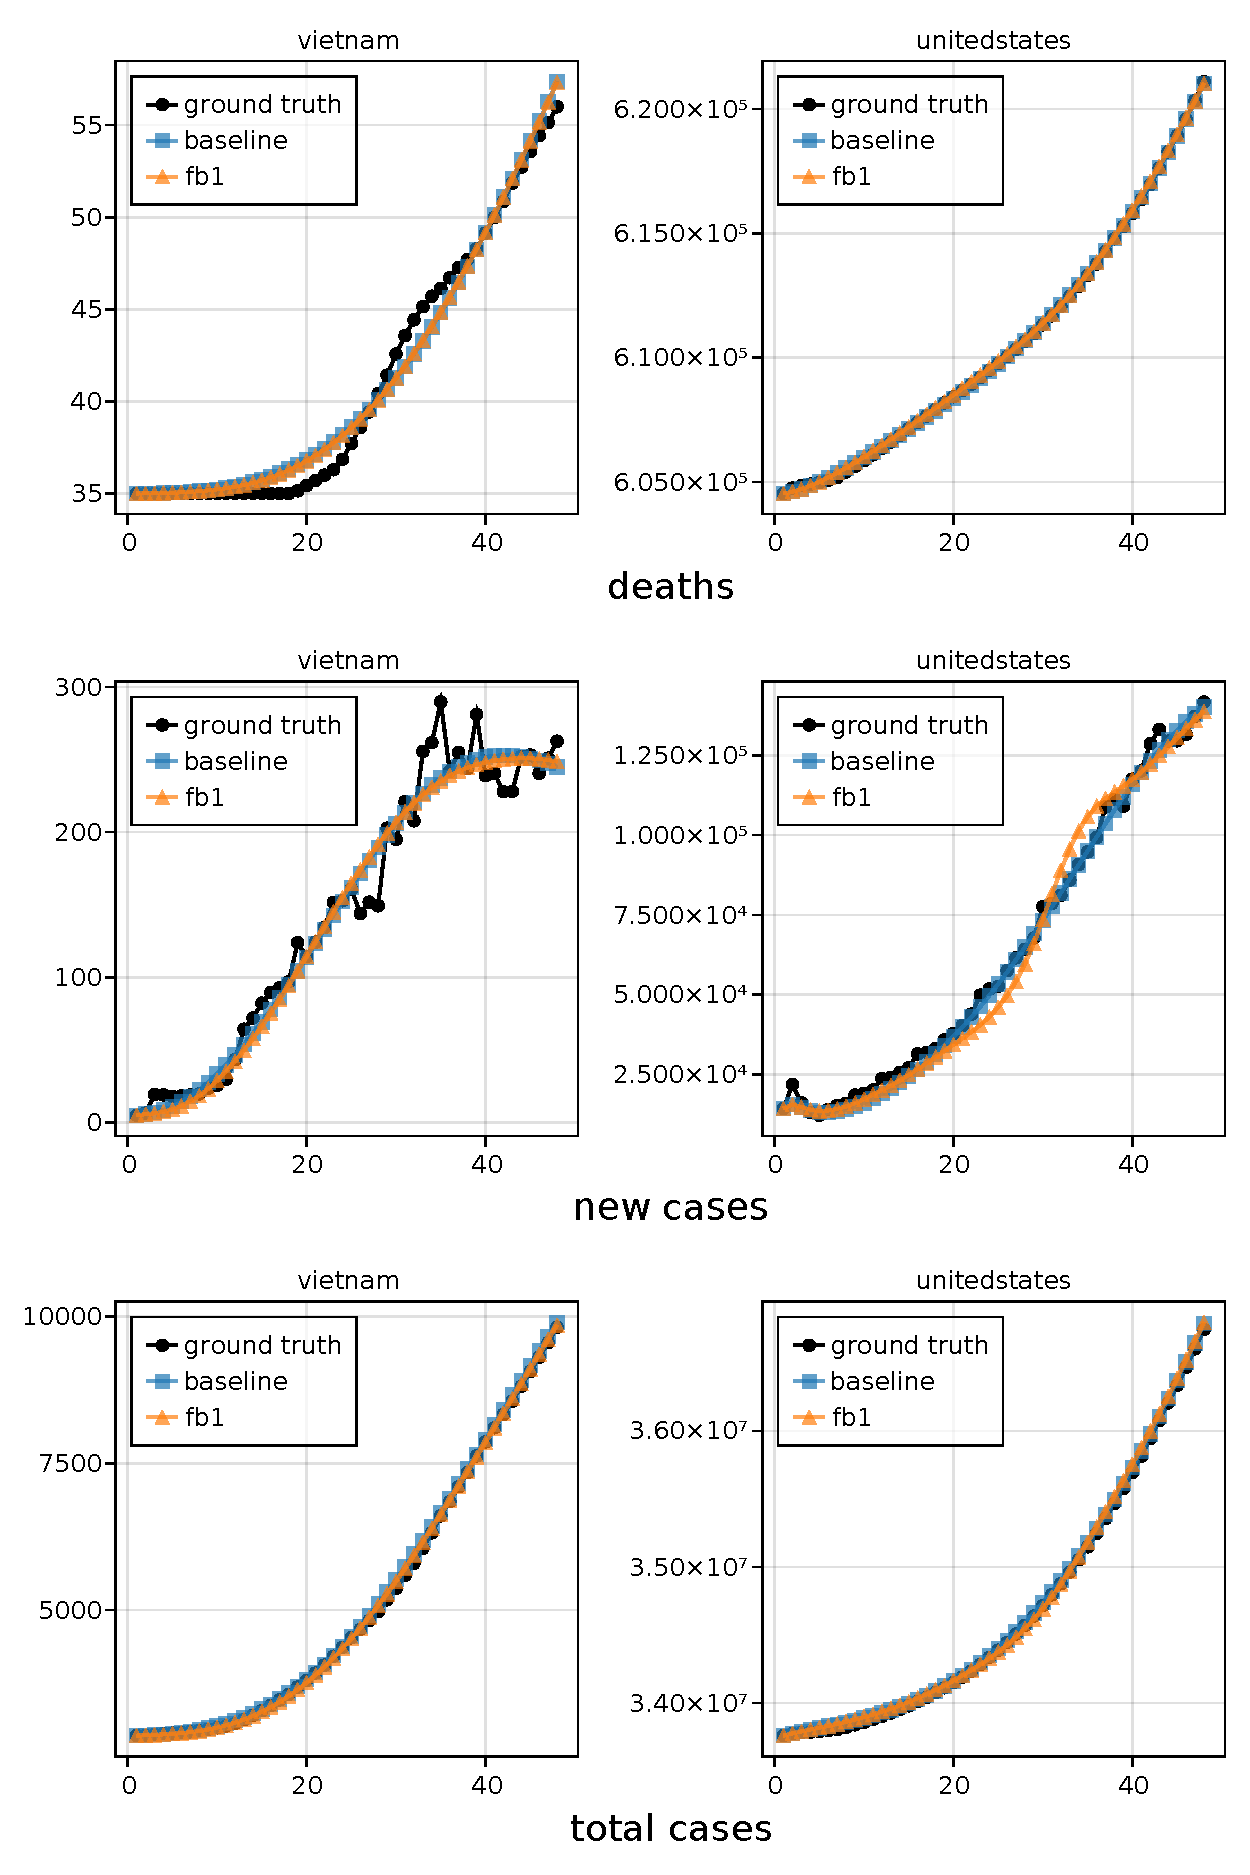
\includegraphics[scale=0.7]{fit_country_level.pdf}
    \caption{Predictions made by all versions of the model for the training period after having trained with country-level data. Each row contains the predictions for a compartment for each of the considered countries. Here the second version is denoted as \textit{fb1}}
    \label{fig:fit-country-level}
\end{figure}

\begin{figure}[!htb]
    \centering
    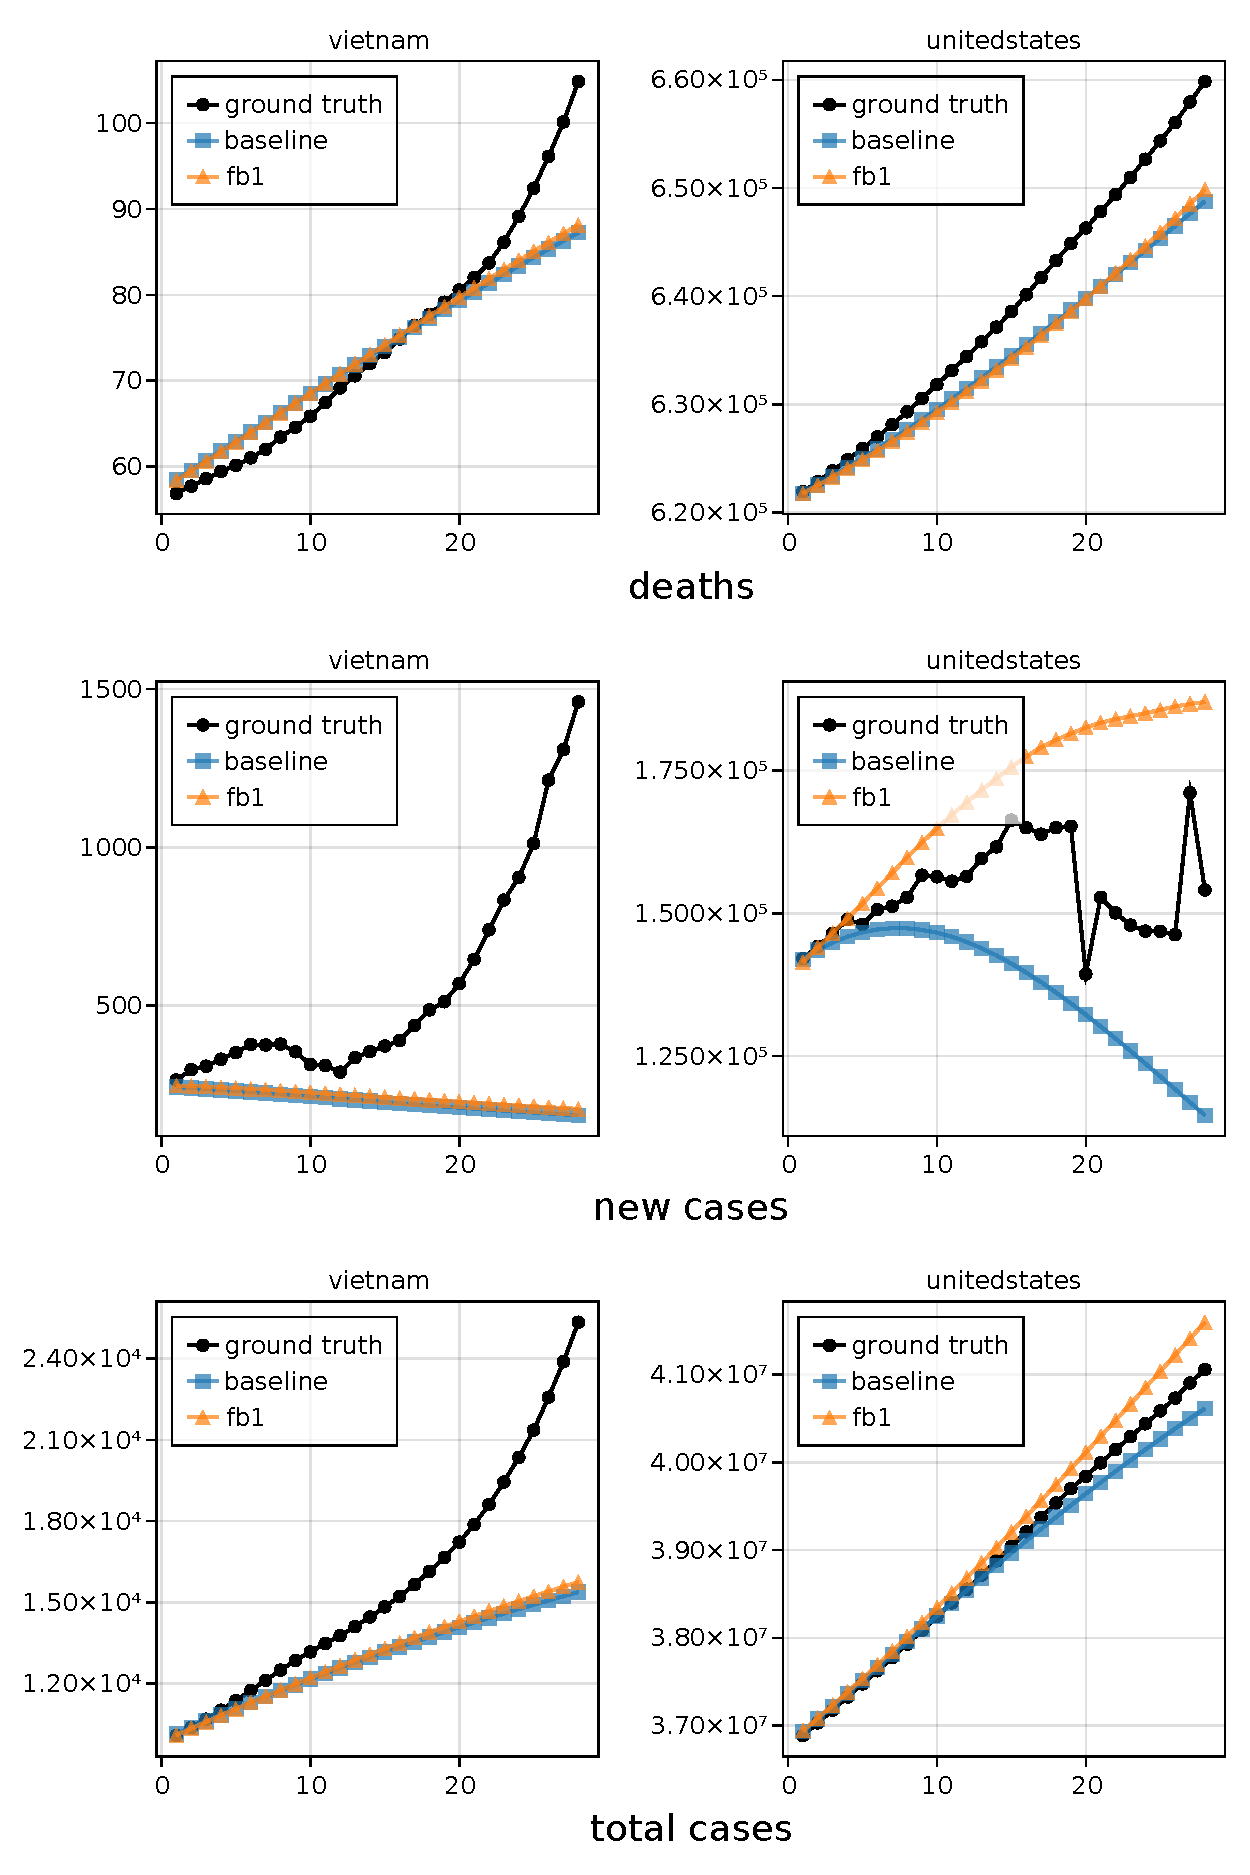
\includegraphics[scale=0.7]{pred_country_level.pdf}
    \caption{Predictions made by all versions of the model for the testing period after having trained with country-level data. Each row contains the predictions for a compartment for each of the considered countries. Here the second version is denoted as \textit{fb1}}
    \label{fig:pred-country-level}
\end{figure}

\begin{figure}[!htb]
    \centering
    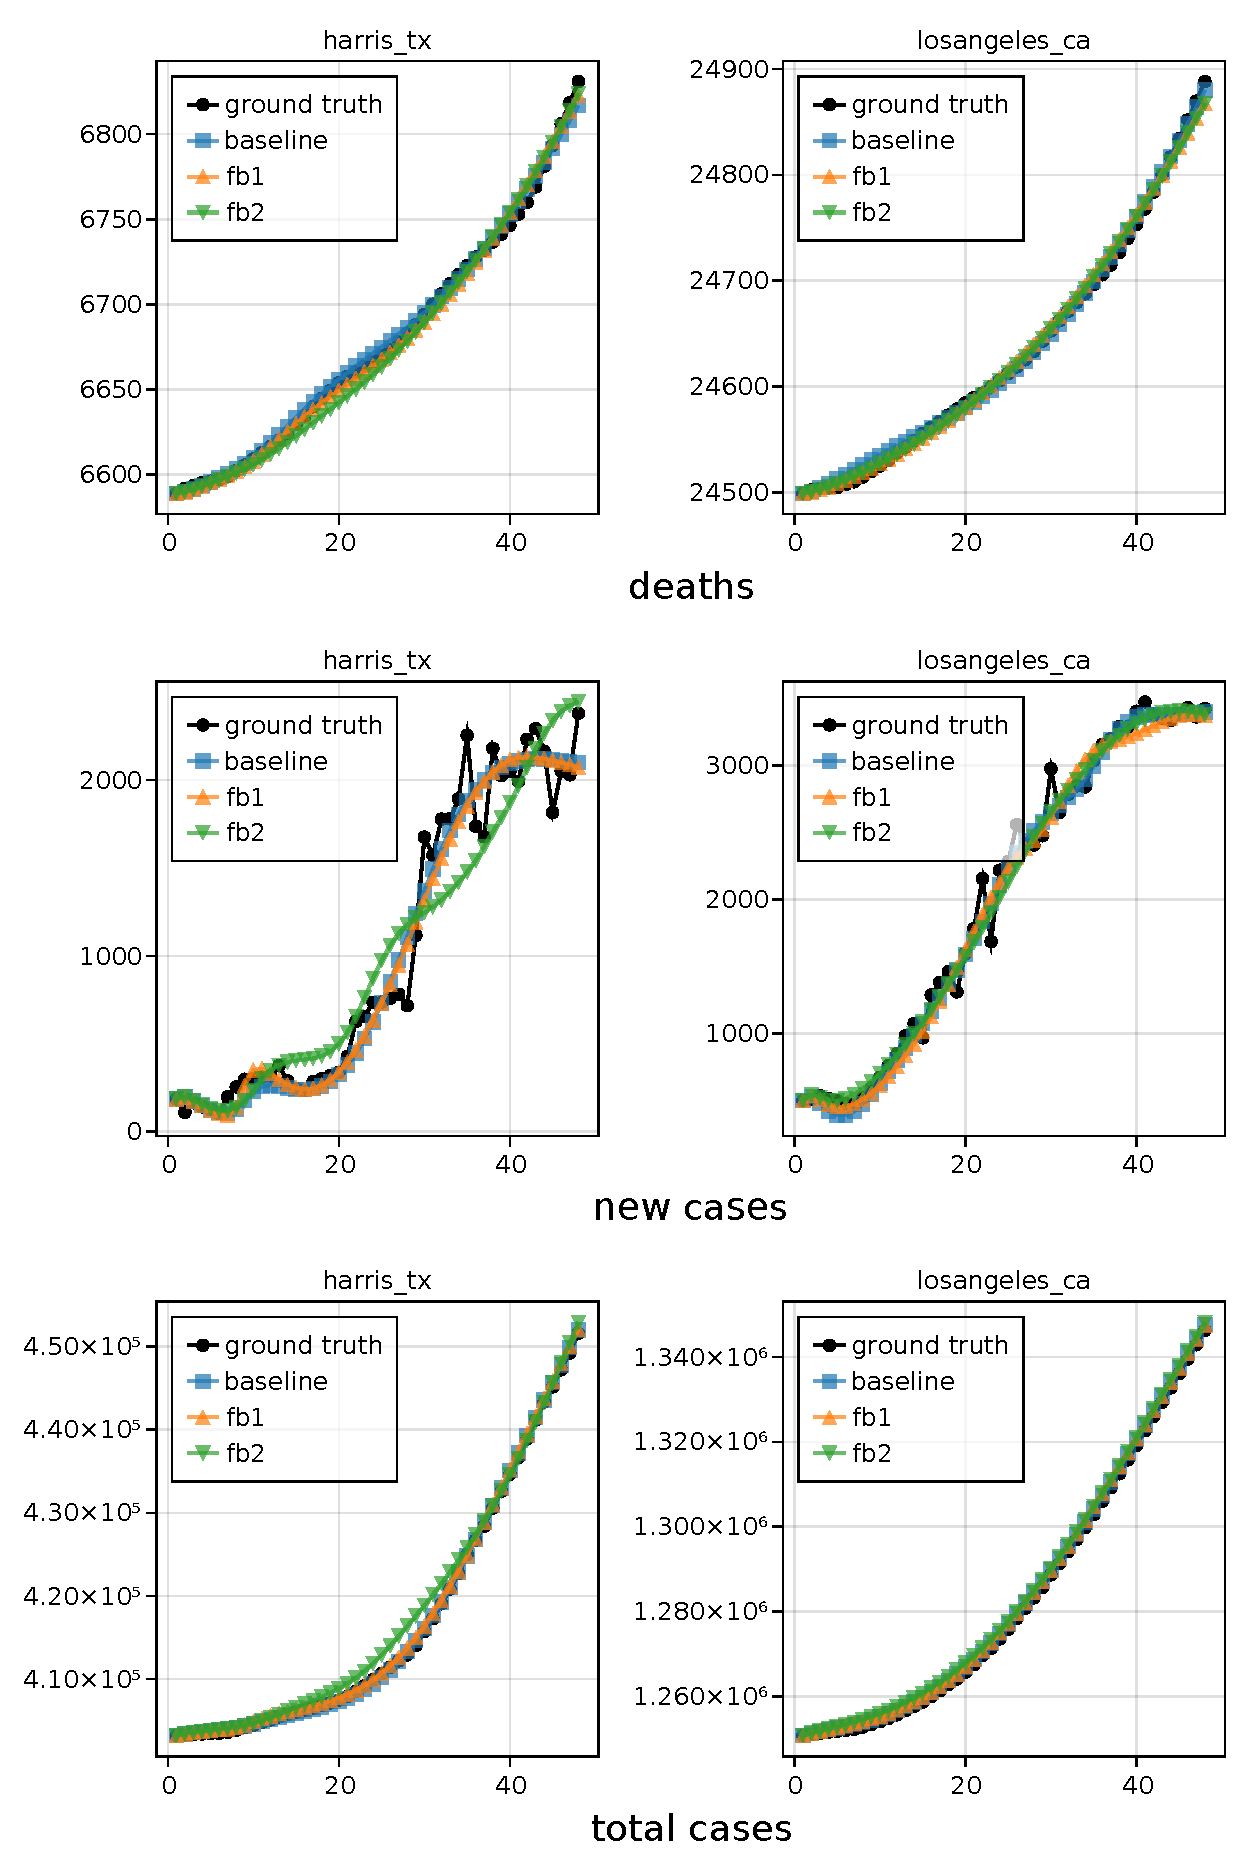
\includegraphics[scale=0.7]{fit_us_counties1.pdf}
    \caption{Predictions made by all versions of the model for the training period after having trained with data for Harris (Texas) and Los Angeles (California). Each row contains the predictions for a compartment for each of the considered counties. Here the second version is denoted as \textit{fb1} and the third version is denoted as \textit{fb2}}
    \label{fig:fit-us-counties1}
\end{figure}

\begin{figure}[!htb]
    \centering
    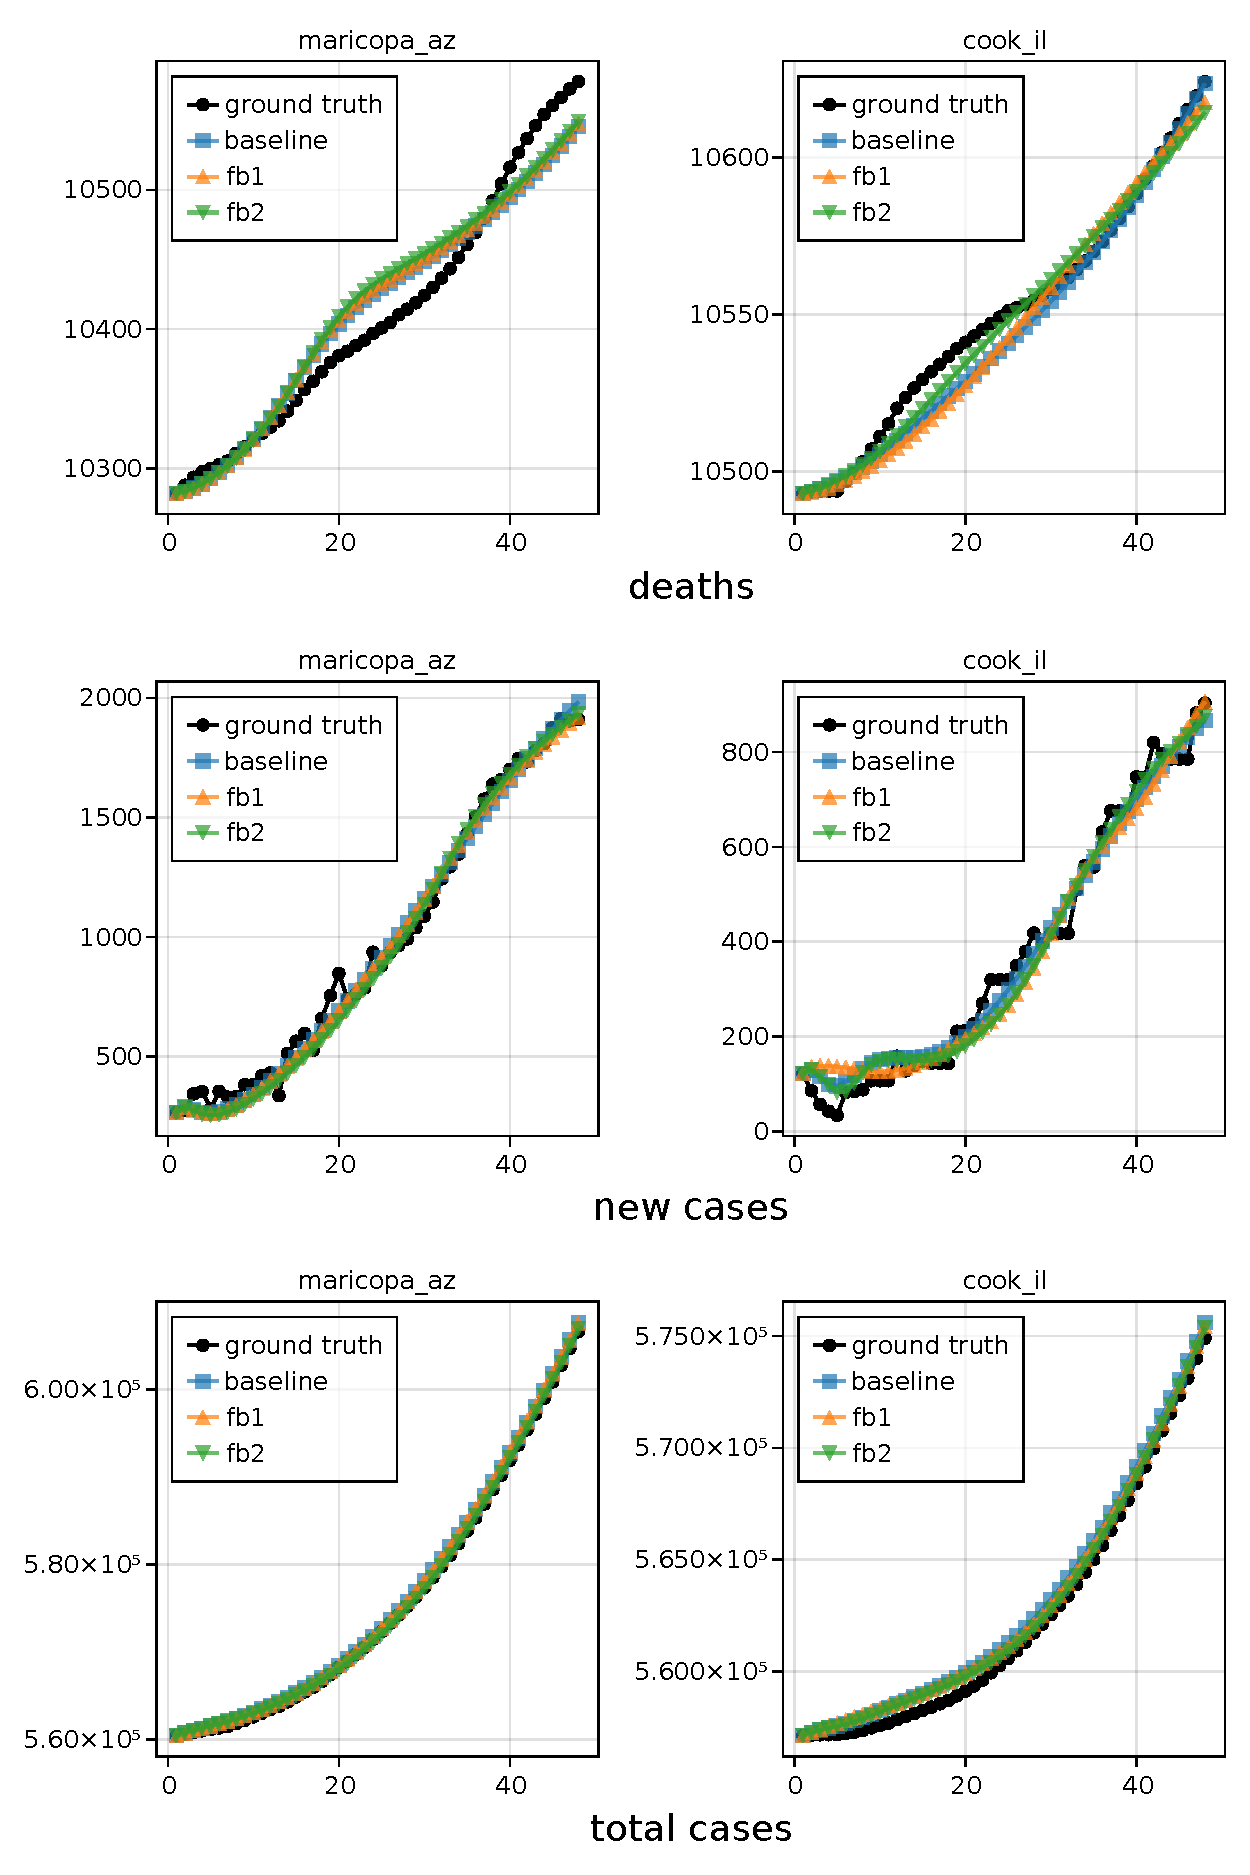
\includegraphics[scale=0.7]{fit_us_counties2.pdf}
    \caption{Predictions made by all versions of the model for the training period after having trained with data for Maricopa (Arizona) and Cook (Illinois). Each row contains the predictions for a compartment for each of the considered counties. Here the second version is denoted as \textit{fb1} and the third version is denoted as \textit{fb2}}
    \label{fig:fit-us-counties2}
\end{figure}

\begin{figure}[!htb]
    \centering
    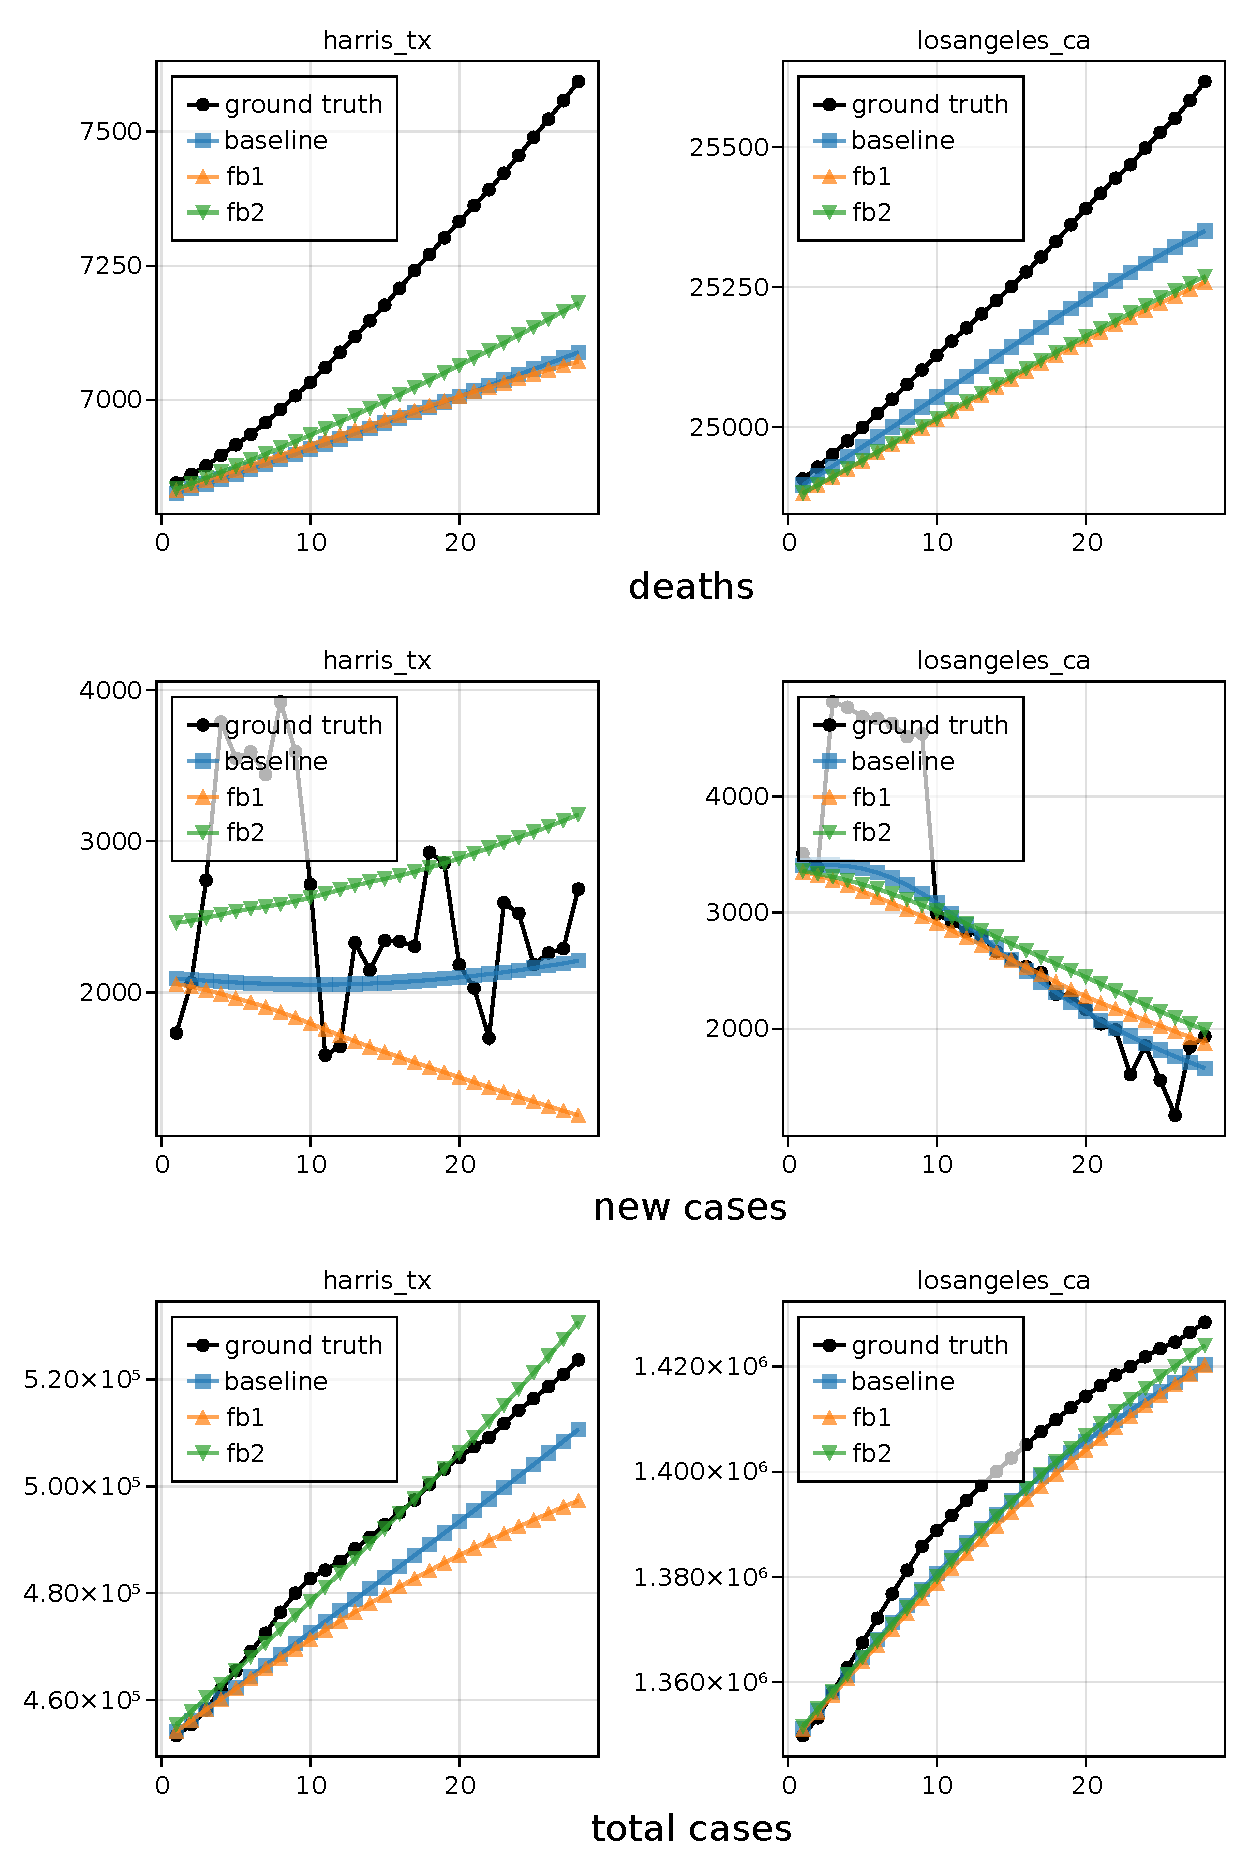
\includegraphics[scale=0.7]{pred_us_counties1.pdf}
    \caption{Predictions made by all versions of the model for the testing period after having trained with data for Harris (Texas) and Los Angeles (California). Each row contains the predictions for a compartment for each of the considered counties. Here the second version is denoted as \textit{fb1} and the third version is denoted as \textit{fb2}}
    \label{fig:pred-us-counties1}
\end{figure}

\begin{figure}[!htb]
    \centering
    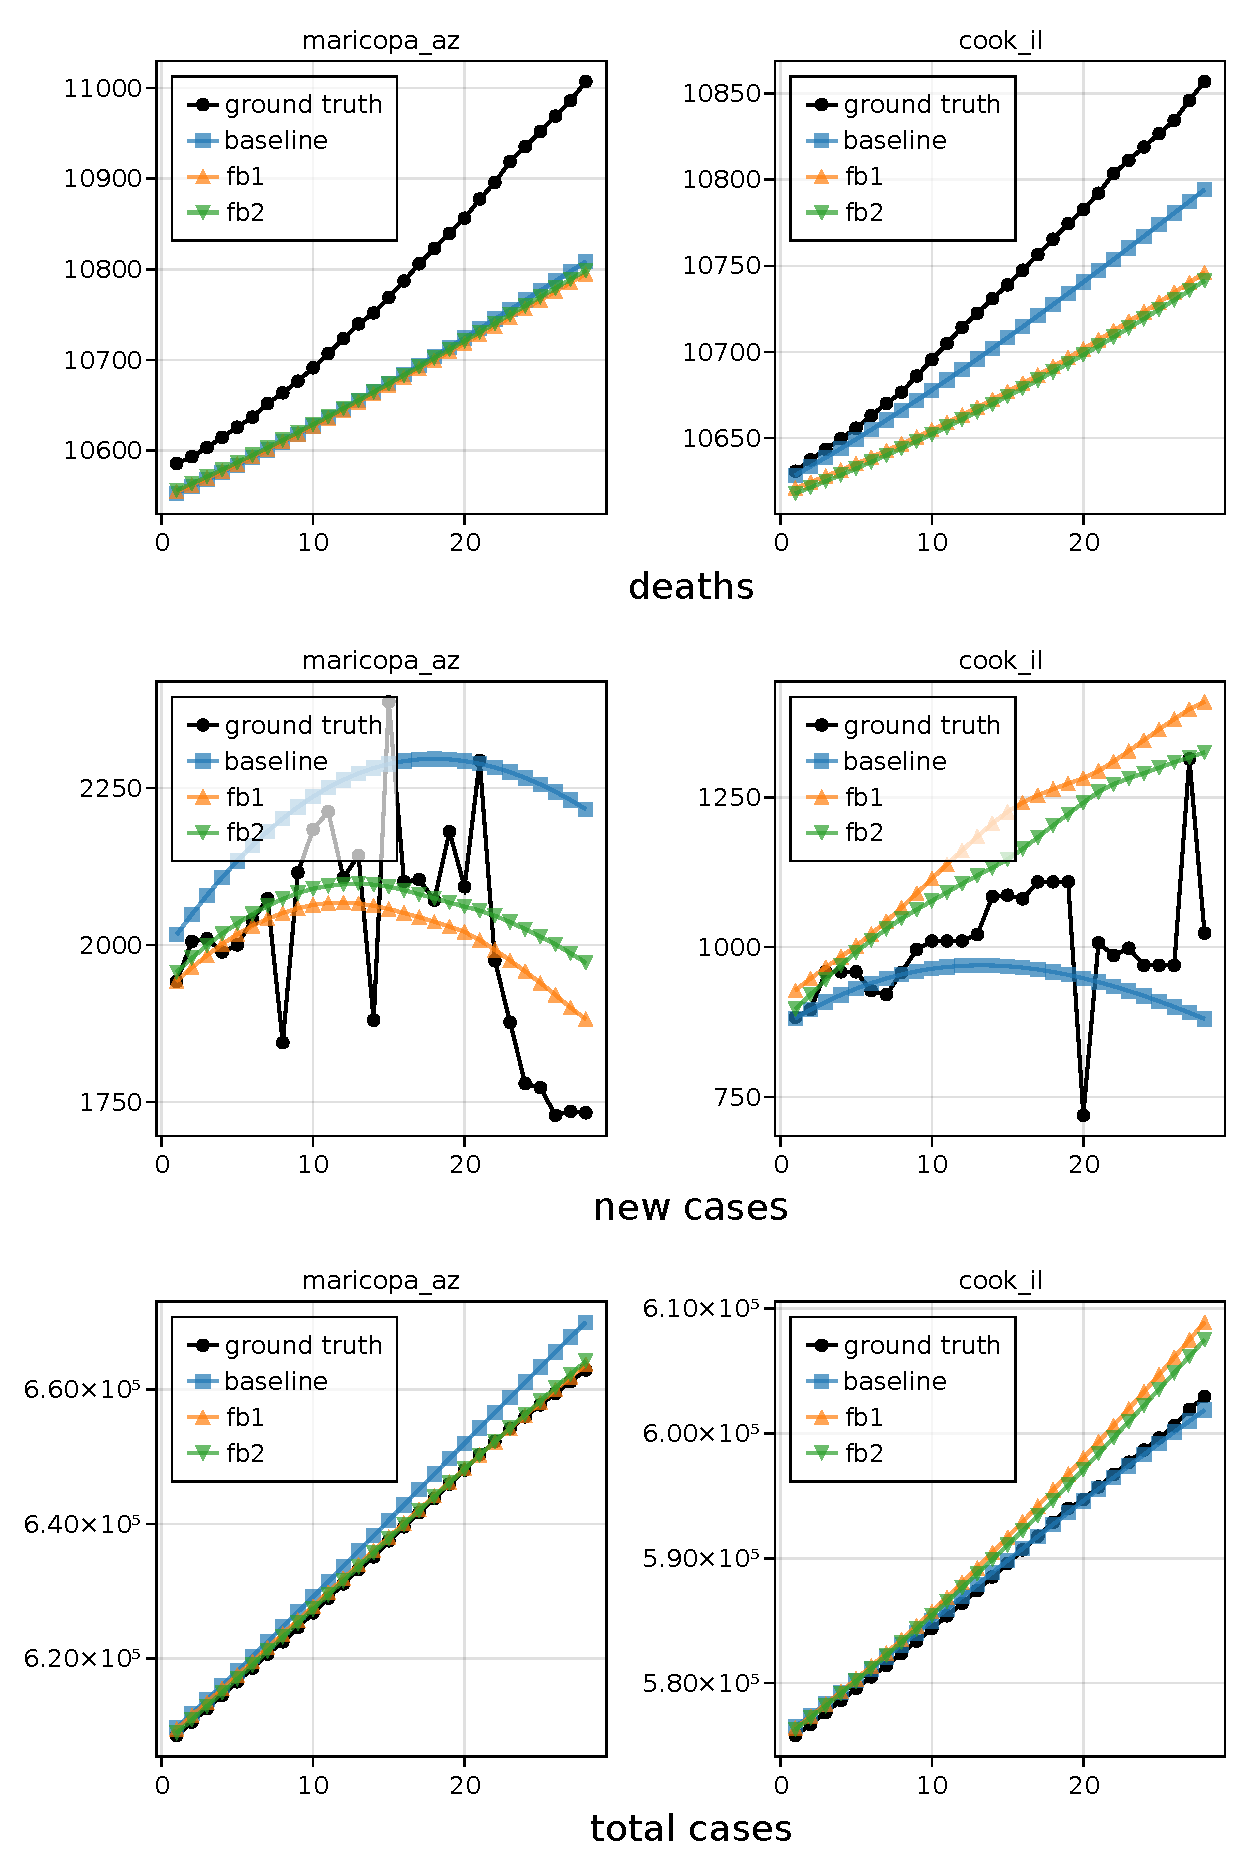
\includegraphics[scale=0.7]{pred_us_counties2.pdf}
    \caption{Predictions made by all versions of the model for the testing period after having trained with data for Maricopa (Arizona) and Cook (Illinois). Each row contains the predictions for a compartment for each of the considered counties. Here the second version is denoted as \textit{fb1} and the third version is denoted as \textit{fb2}}
    \label{fig:pred-us-counties2}
\end{figure}

\begin{figure}[!htb]
    \centering
    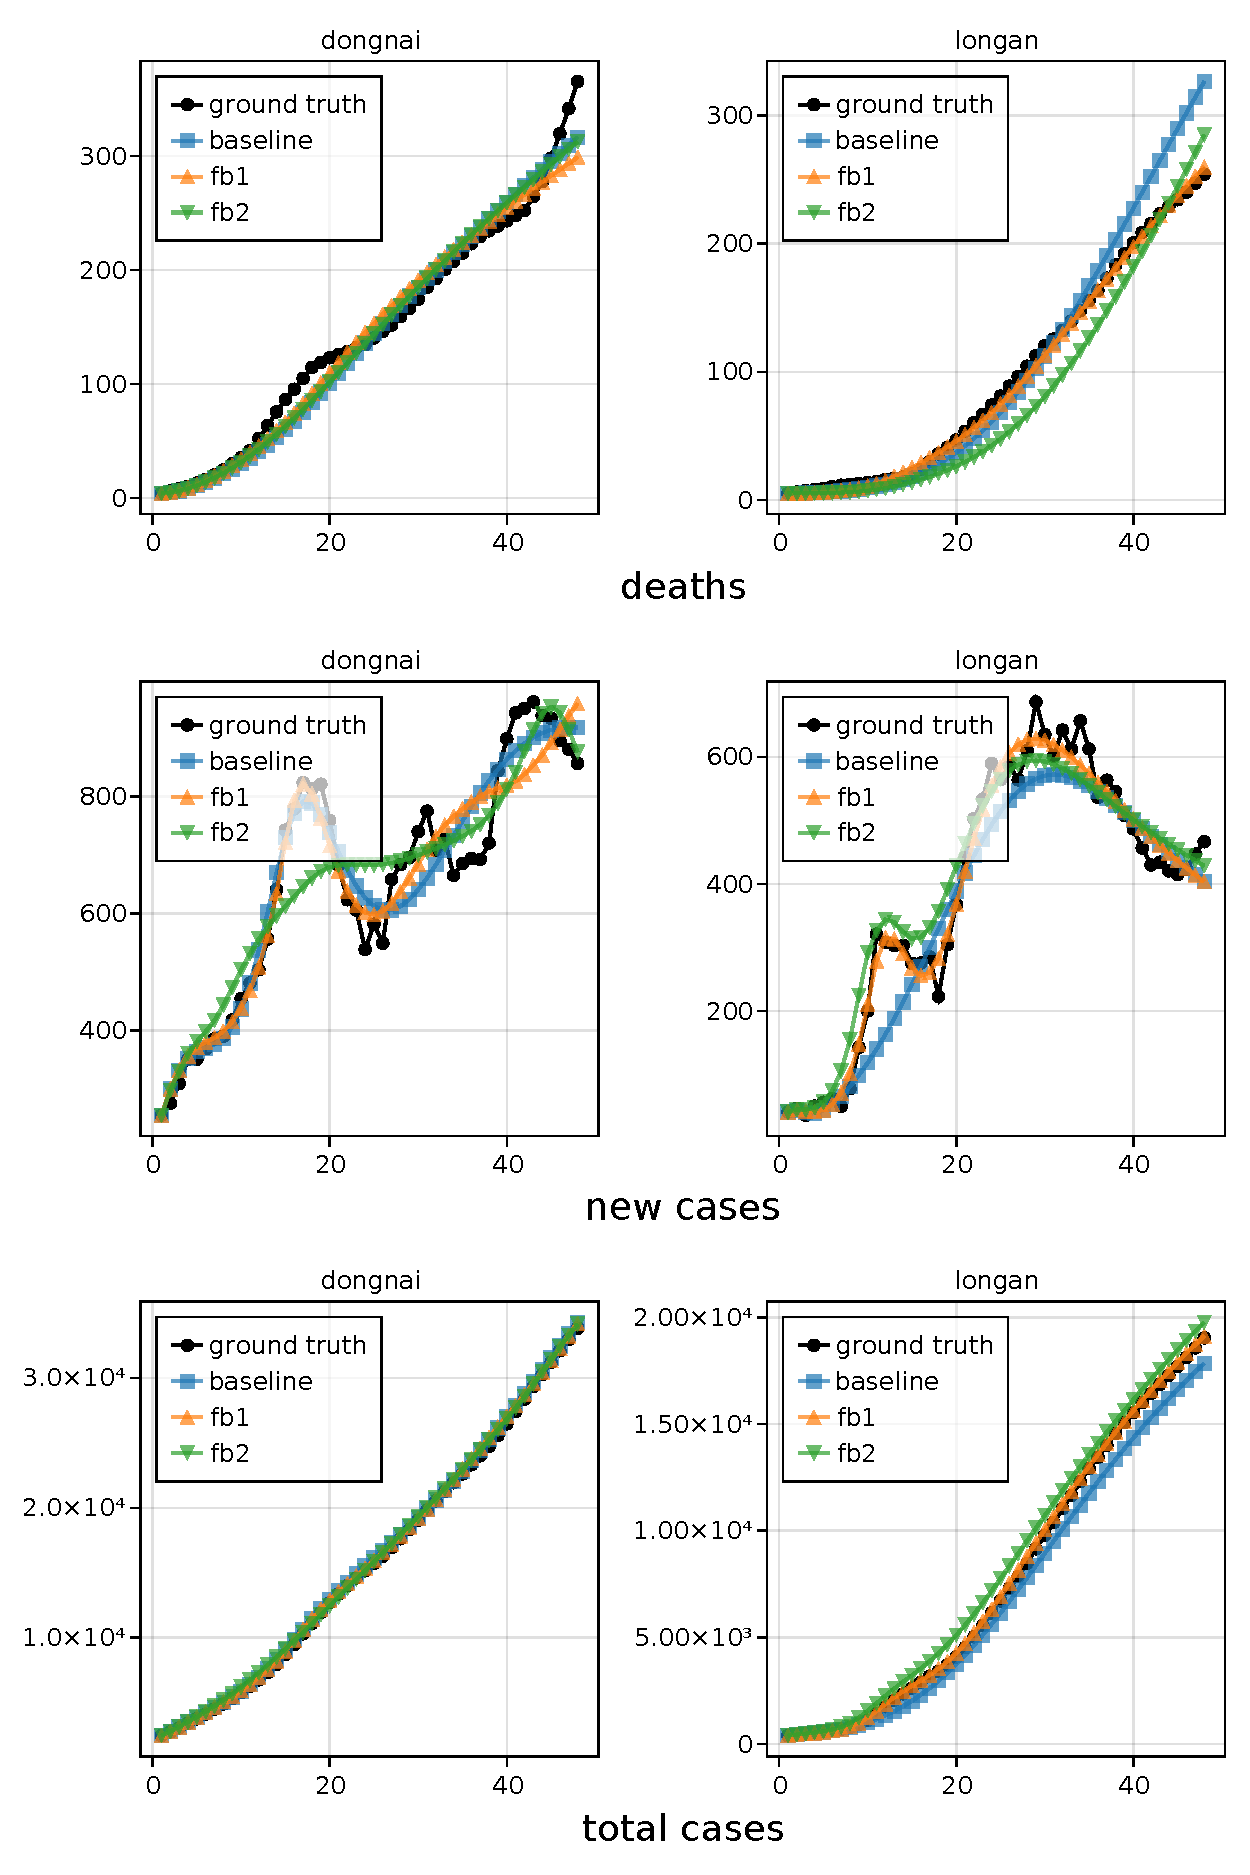
\includegraphics[scale=0.7]{fit_vn_provinces1.pdf}
    \caption{Predictions made by all versions of the model for the training period after having trained with data for Dong Nai and Long An. Each row contains the predictions for a compartment for each of the considered provinces. Here the second version is denoted as \textit{fb1} and the third version is denoted as \textit{fb2}}
    \label{fig:fit-vn-provinces1}
\end{figure}

\begin{figure}[!htb]
    \centering
    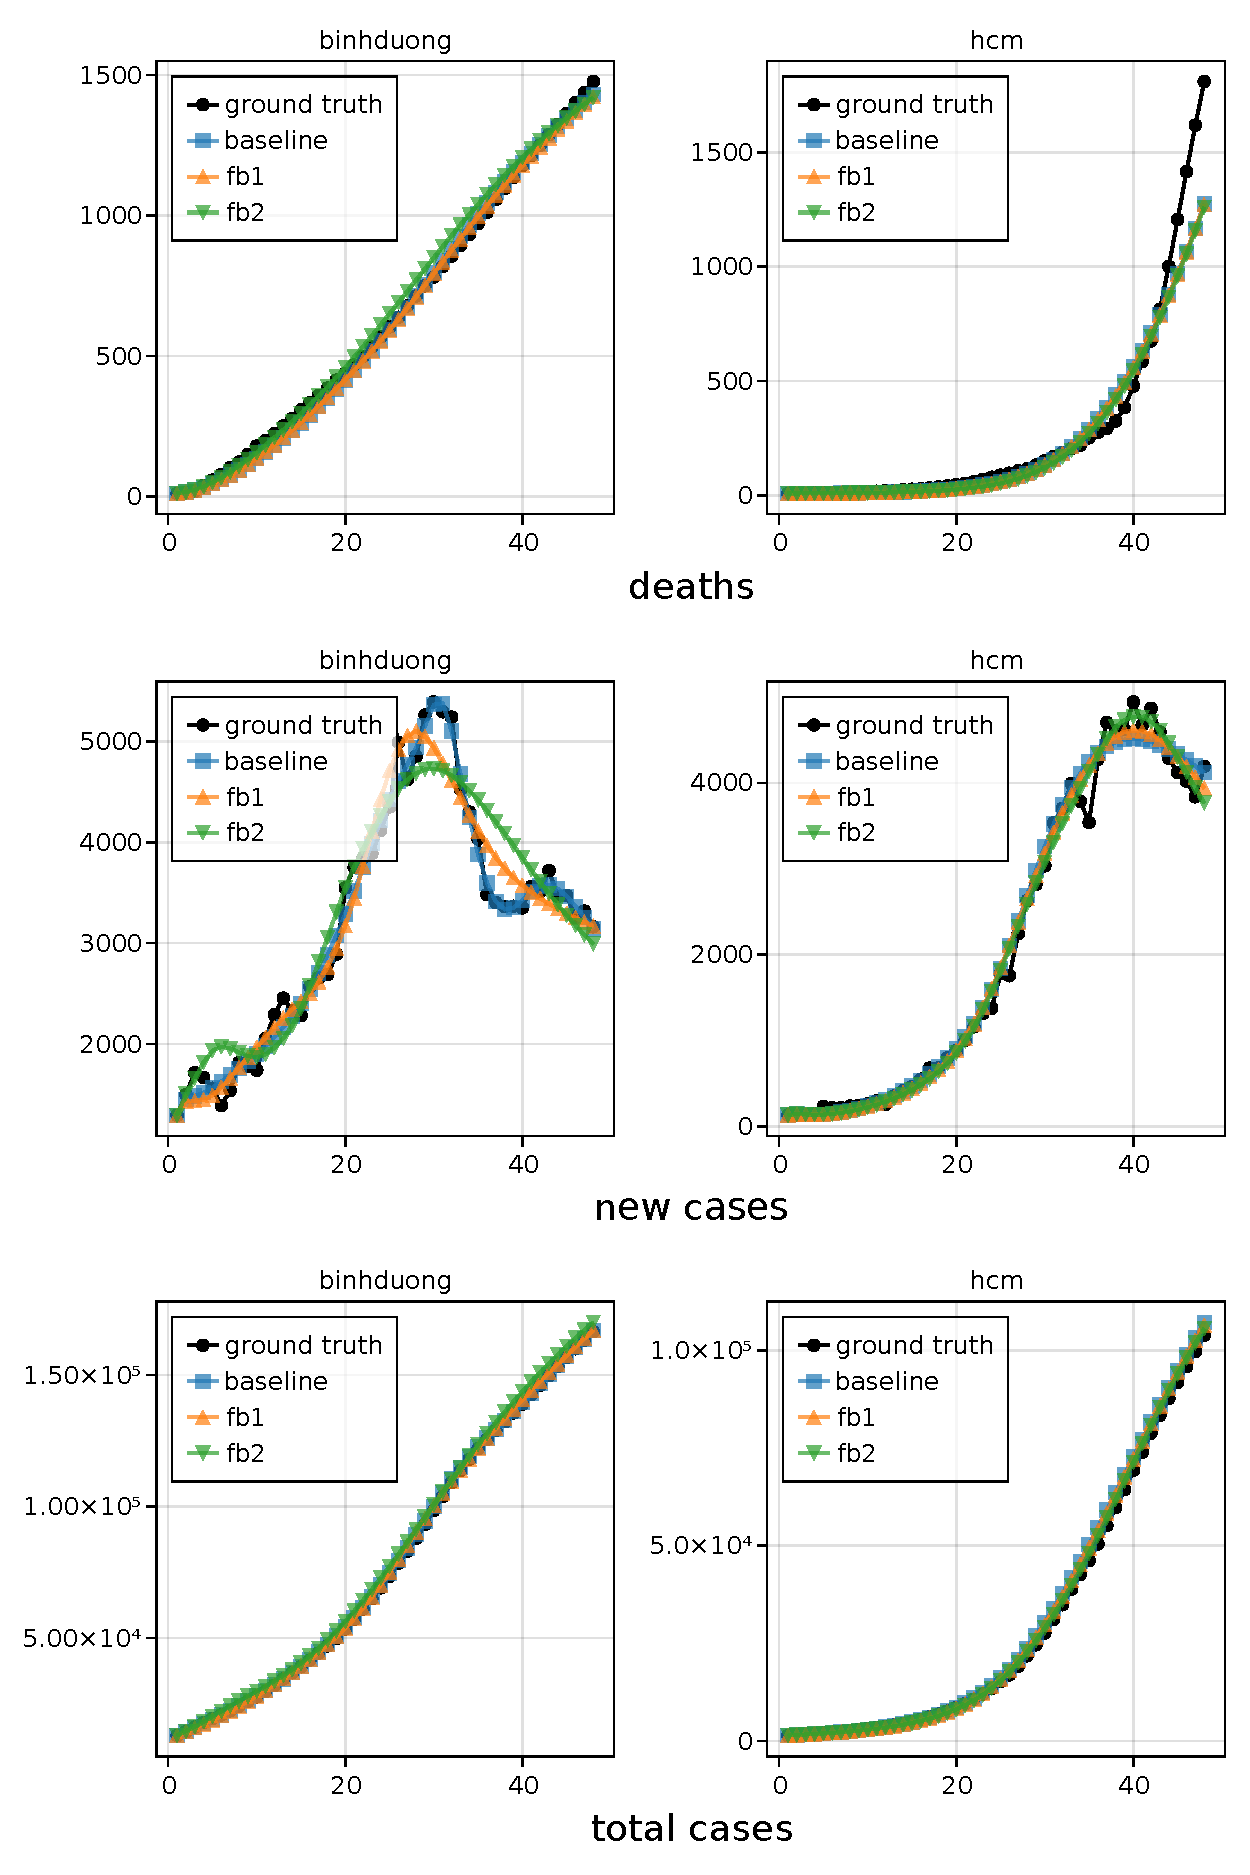
\includegraphics[scale=0.7]{fit_vn_provinces2.pdf}
    \caption{Predictions made by all versions of the model for the training period after having trained with data for Binh Duong and Ho Chi Minh city. Each row contains the predictions for a compartment for each of the considered provinces. Here the second version is denoted as \textit{fb1} and the third version is denoted as \textit{fb2}}
    \label{fig:fit-vn-provinces2}
\end{figure}

\begin{figure}[!htb]
    \centering
    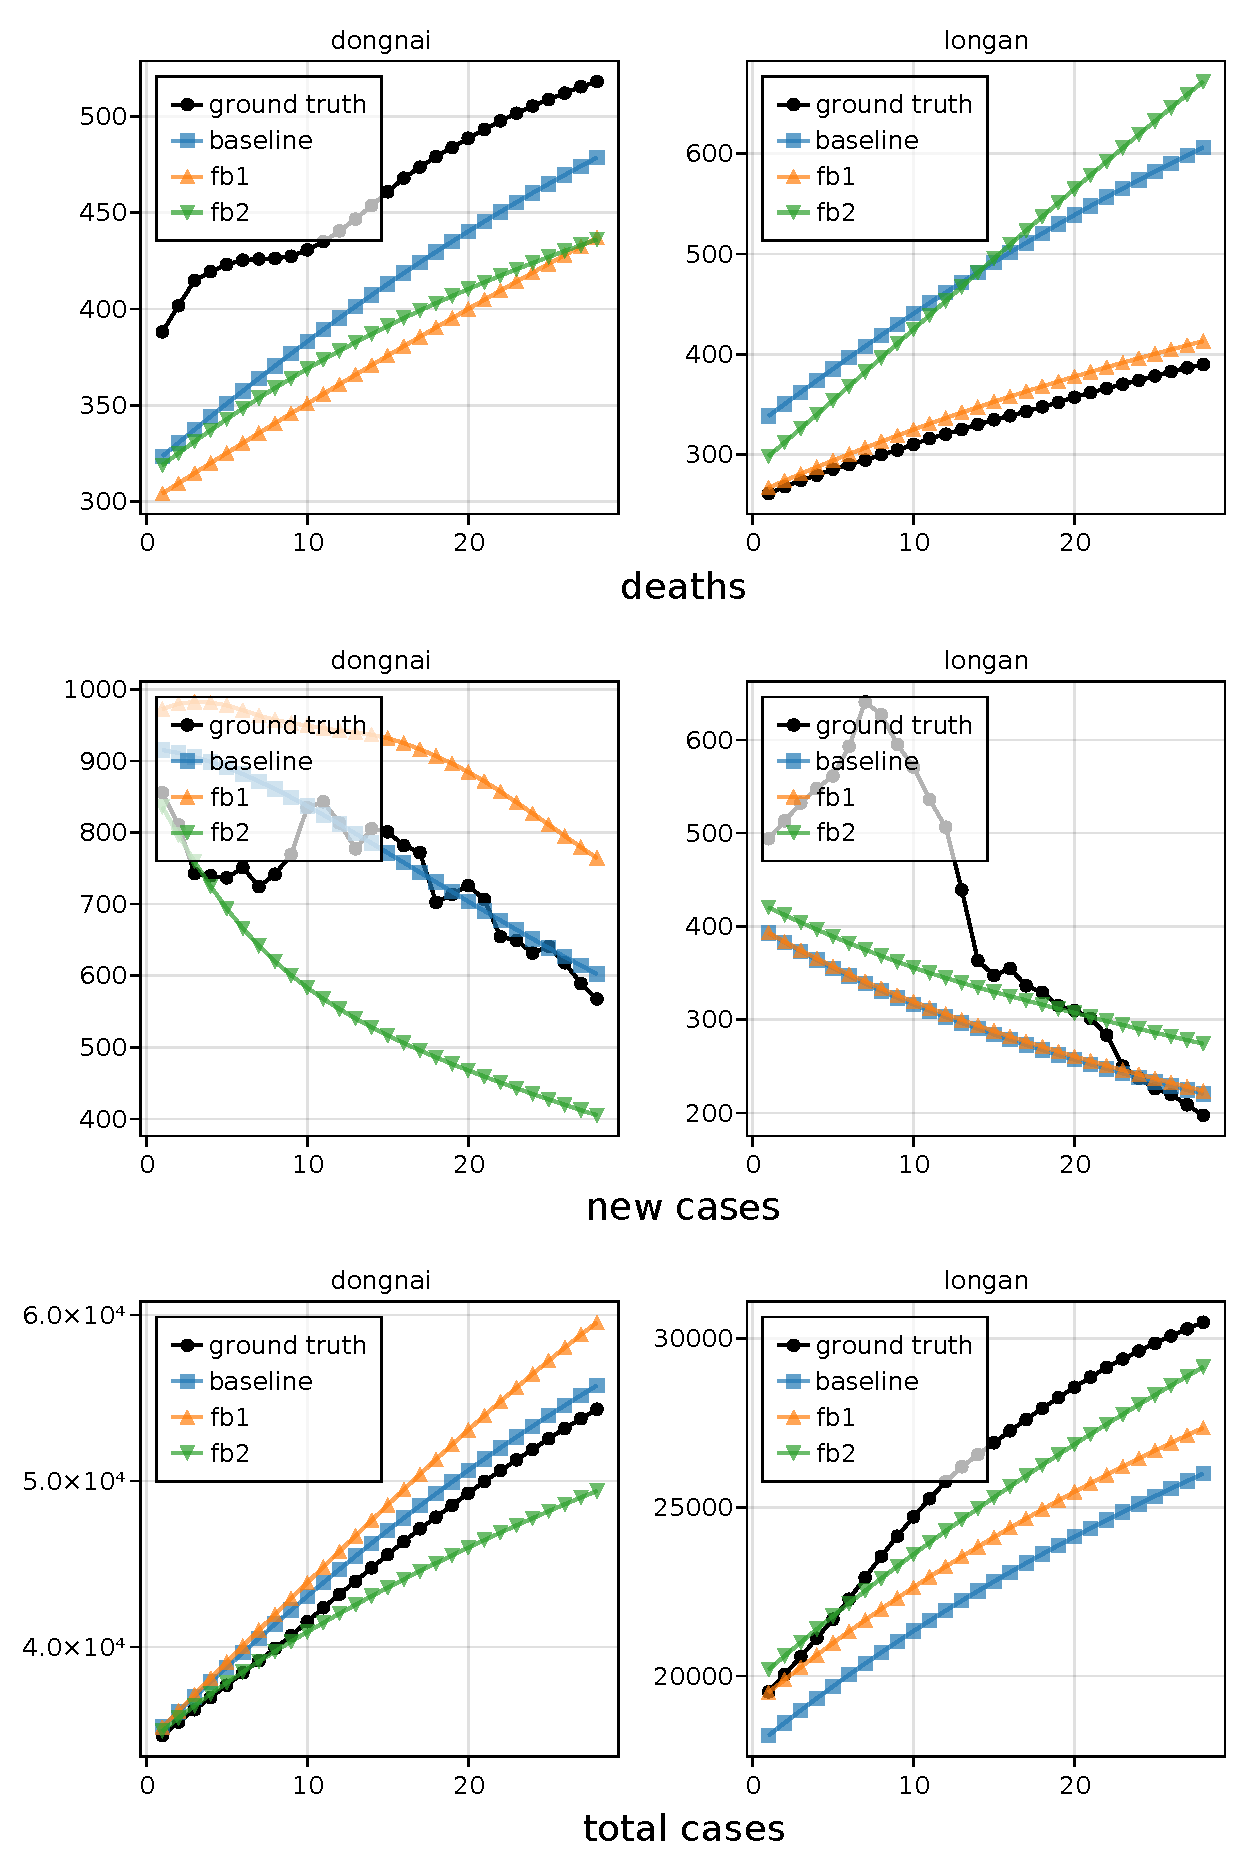
\includegraphics[scale=0.7]{pred_vn_provinces1.pdf}
    \caption{Predictions made by all versions of the model for the testing period after having trained with data for Dong Nai and Long An. Each row contains the predictions for a compartment for each of the considered provinces. Here the second version is denoted as \textit{fb1} and the third version is denoted as \textit{fb2}}
    \label{fig:pred-vn-provinces1}
\end{figure}


\begin{figure}[!htb]
    \centering
    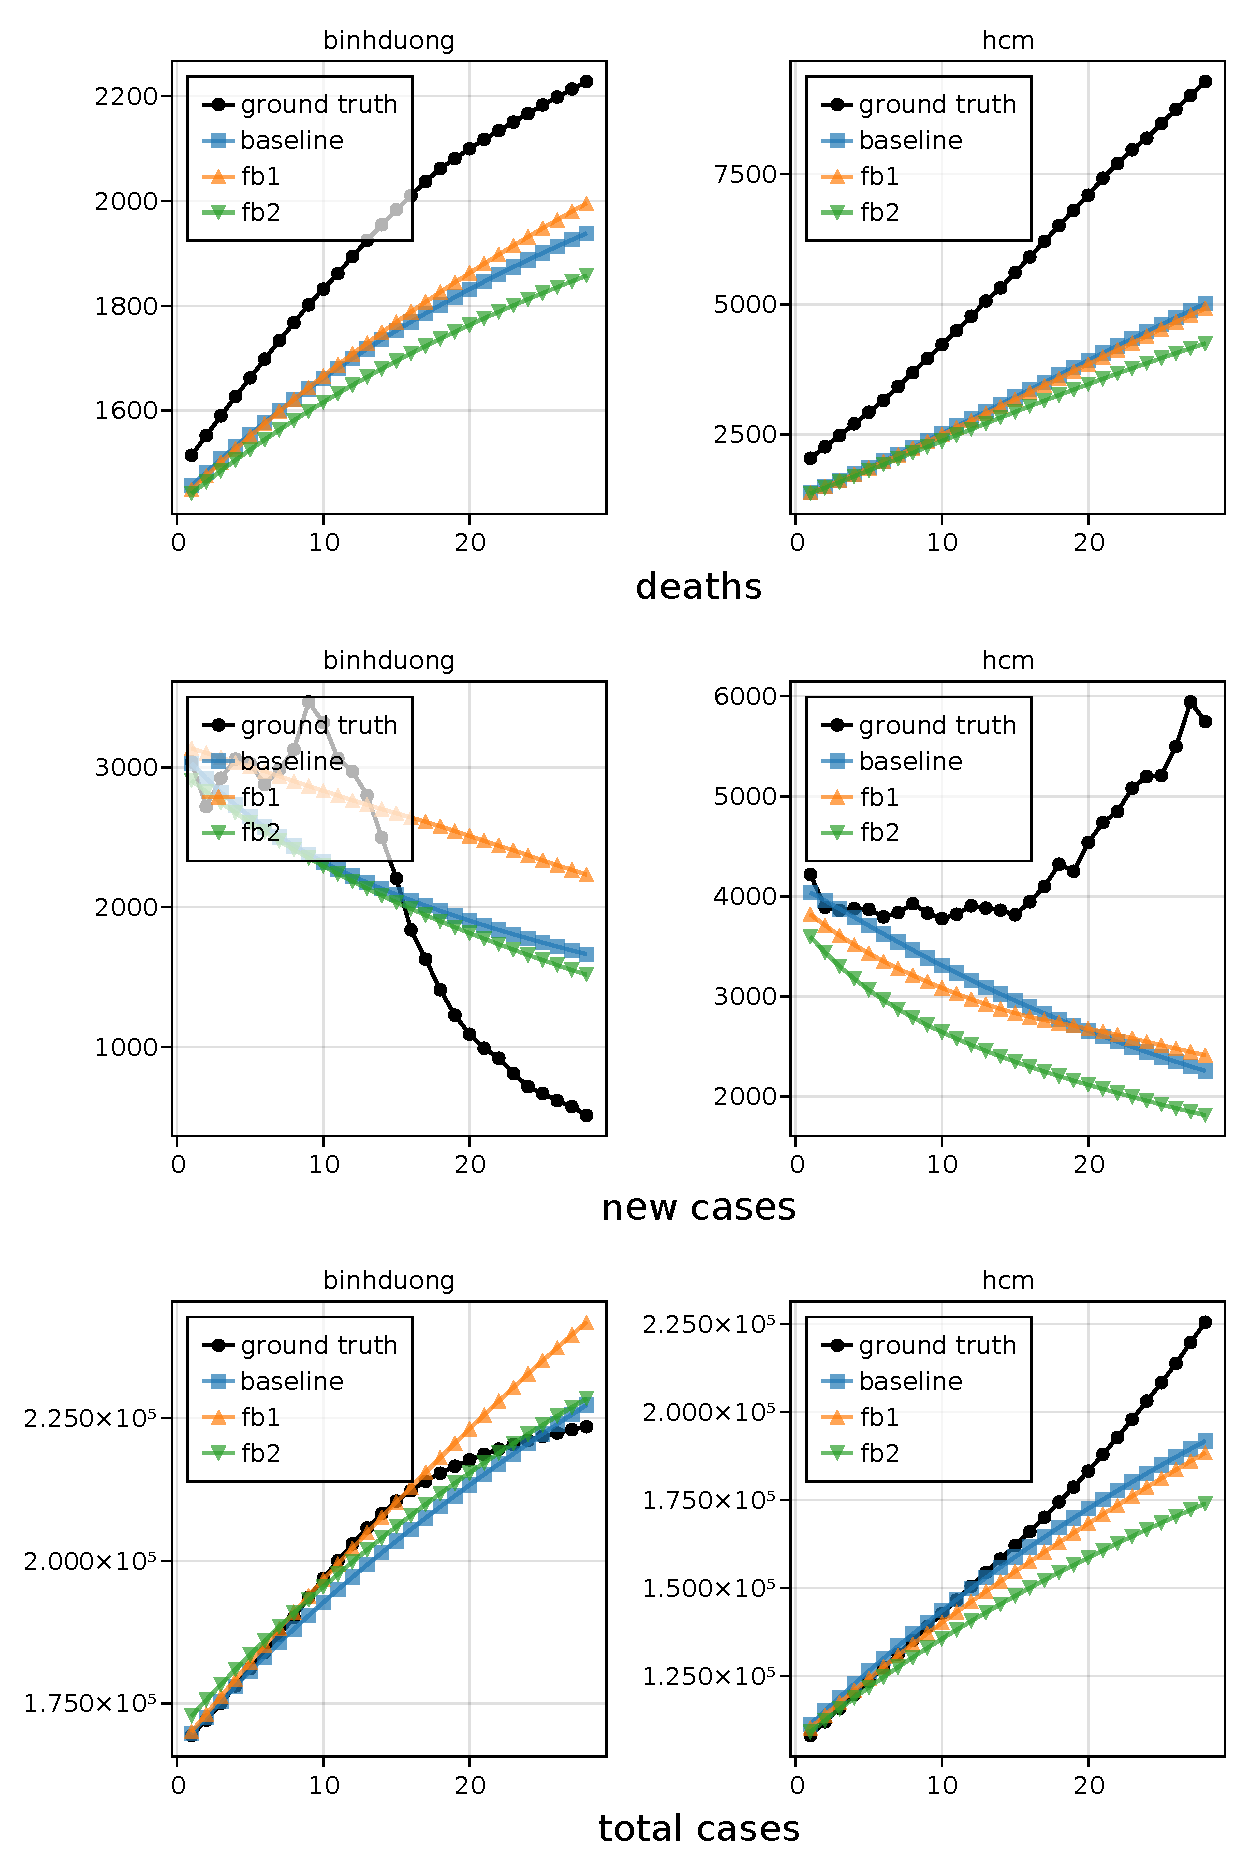
\includegraphics[scale=0.7]{pred_vn_provinces2.pdf}
    \caption{Predictions made by all versions of the model for the testing period after having trained with data for Binh Duong and Ho Chi Minh city. Each row contains the predictions for a compartment for each of the considered provinces. Here the second version is denoted as \textit{fb1} and the third version is denoted as \textit{fb2}}
    \label{fig:pred-vn-provinces2}
\end{figure}

\chapter{Package core implementations}

\begin{figure}[!htb]
\centering
\begin{jllisting}
function SEIRD!(du, u, p, t)
    @inbounds begin
        S, E, I, _, _, N, C, _ = u
        β, γ, λ, α = p
        du[1] = -β * S * I / N
        du[2] = β * S * I / N - γ * E
        du[3] = γ * E - λ * I
        du[4] = (1 - α) * λ * I
        du[5] = α * λ * I
        du[6] = -α * λ * I
        du[7] = -C + γ * E
        du[8] = γ * E
    end
    return nothing
end
\end{jllisting}
\caption{The function that defines the underlying SEIR model, where \textit{du} is a vector that will be modified in-place to contain the system derivatives at each time step, \textit{u} is a vector contains the current state of the system, \textit{p} is a vector contains all the system parameters, and \textit{t} is the value of the current time step.}
\label{fig:diffeq-seird-inplace}
\end{figure}

\begin{figure}[!htb]
\begin{jllisting}
function experiment_loss_sse(min::AbstractVector{R},
                             max::AbstractVector{R},
                             ζ::R) where {R<:Real}
    scale = max .- min
    lossfn = function (ŷ::AbstractArray{R}, y, tsteps) where {R<:Real}
        s = zero(R)
        sz = size(y)
        @inbounds for j in 1:sz[2], i in 1:sz[1]
            s += ((ŷ[i, j] - y[i, j]) / scale[i])^2 / sz[2] * exp(ζ * tsteps[j])
        end
        return s
    end
    return lossfn
end

min = vec(minimum(train_dataset.data; dims=2))
max = vec(maximum(train_dataset.data; dims=2))
lossfn_inner = experiment_loss_sse(min, max, loss_time_weighting)

lossfn = function (ŷ, y, params, tsteps)
    pnamed = namedparams(model, params)
    return lossfn_inner(ŷ, y, tsteps) +
            loss_regularization / (2 * size(y, 2)) *
            (sum(abs2, pnamed.θ1) + sum(abs2, pnamed.θ2))
end
\end{jllisting}
\caption{The implementation for the loss function defined by \autoref{eq:ude-model-loss}. Here, \textit{lossfn\_inner} is a closure that is used for calculating the loss value with min-max scaling and time weighting, and \textit{lossfn} is a closure that is used for calculating the loss value regularized with the \glspl{ANN} parameters. These two steps are separated because how the \gls{ANN} parameters are arranged within system parameters \textit{params} can be different among different versions of the model.}
\label{fig:diffeq-seird-experiment-loss}
\end{figure}

\begin{figure}[!htb]
\centering
\begin{jllisting}
struct SEIRDFbMobility2{ANN1<:FastChain,
                        ANN2<:FastChain,
                        T<:Real,
                        DS<:AbstractMatrix{T}} <: AbstractCovidModel
    β_ann::ANN1
    α_ann::ANN2
    β_ann_paramlength::Int
    α_ann_paramlength::Int
    β_bounds::Tuple{T,T}
    γ_bounds::Tuple{T,T}
    λ_bounds::Tuple{T,T}
    α_bounds::Tuple{T,T}
    population::T
    time_scale::T
    movement_range_data::DS
    social_proximity_data::DS

    function SEIRDFbMobility2(
        β_bounds::Tuple{T,T},
        γ_bounds::Tuple{T,T},
        λ_bounds::Tuple{T,T},
        α_bounds::Tuple{T,T},
        population::T,
        time_scale::T,
        movement_range_data::DS,
        social_proximity_data::DS,
    ) where {T<:Real,DS<:AbstractMatrix{T}}
        β_ann = FastChain(
            StaticDense(7, 8, mish, initW = Flux.glorot_normal),
            StaticDense(8, 8, mish, initW = Flux.glorot_normal),
            StaticDense(8, 8, mish, initW = Flux.glorot_normal),
            StaticDense(8, 1,
                        x -> boxconst(x, β_bounds),
                        initW = Flux.glorot_normal),
        )
        α_ann = FastChain(
            StaticDense(4, 8, mish, initW = Flux.glorot_normal),
            StaticDense(8, 1,
                        x -> boxconst(x, α_bounds),
                        initW = Flux.glorot_normal),
        )
        return new{typeof(β_ann),typeof(α_ann),T,DS}(
            β_ann, α_ann,
            DiffEqFlux.paramlength(β_ann),
            DiffEqFlux.paramlength(α_ann),
            β_bounds, γ_bounds, λ_bounds, α_bounds, population,
            time_scale,
            movement_range_data,
            social_proximity_data,
        )
    end
end
\end{jllisting}
\caption{The third version of the model represented by a Julia struct that holds all the necessary objects and data for modelling the disease a location. \textit{$\beta\_ann$} and \textit{$\alpha\_ann$} are the object that represent the \glspl{ANN}, and \textit{$\beta\_ann\_paramlength$} and \textit{$\alpha\_ann\_paramlength$} are the number of parameters used by each of the \gls{ANN}, respectively. \textit{$\beta\_bounds$}, \textit{$\gamma\_bounds$}, \textit{$\lambda\_bounds$}, and \textit{$\alpha\_bounds$} are the lower and upper bounds constraints of the parameters. \textit{population} is the population of the modelled location, \textit{time\_scale} is length of the modeled time span, \textit{movement\_range\_data} is a matrix holding the Movement Range Maps data, and \textit{social\_proximity\_data} is a matrix holding the \gls{SPC} indices. The two other versions were defined with similar structures, but the baseline version did not contain the fields for the covariates and the second version did not contain the field for the \gls{SPC} index.}
\label{fig:diffeq-seird-fb2-struct}
\end{figure}

\begin{figure}[!htb]
\centering
\begin{jllisting}
function (model::SEIRDFbMobility2)(du, u, p, t)
    @inbounds begin
        time_idx = Int(floor(t + 1))
        # states and params
        S, E, I, R, D, N, _, _ = u
        pnamed = namedparams(model, p)
        # infection rate depends on time, susceptible, and infected
        β = first(
            model.β_ann(
                SVector{7}(
                    t / model.time_scale,
                    S / N, E / N, I / N,
                    model.movement_range_data[1, time_idx],
                    model.movement_range_data[2, time_idx],
                    model.social_proximity_data[1, time_idx],
                ),
                pnamed.θ1,
            ),
        )
        α = first(
            model.α_ann(SVector{4}(t / model.time_scale,
                                   I / N, R / N, D / N),
                        pnamed.θ2)
        )
        SEIRD!(du, u, SVector{4}(β, pnamed.γ, pnamed.λ, α), t)
    end
    return nothing
end
\end{jllisting}
\caption{The definition of a proxy function around the function shown in \autoref{fig:diffeq-seird-inplace} that utilized the ability to make a function call on an object in Julia. Here, \textit{model} is the object that is invoked, \textit{du} is a vector that will be modified in-place to contain the system derivatives at each time step, \textit{u} is a vector contains the current state of the system, \textit{p} is a vector contains all the system parameters, and \textit{t} is the value of the current time step. Unlike in \autoref{fig:diffeq-seird-inplace} where \textit{p} is the parameters for the SEIR model, in this function, \textit{p} is the parameters of the \gls{UDE} which included the weights and biases of the \glspl{ANN}.}
\label{fig:diffeq-seird-fb2}
\end{figure}

\begin{figure}[!htb]
\begin{jllisting}
struct Predictor{
    P<:SciMLBase.DEProblem,
    SO<:SciMLBase.DEAlgorithm,
    SE<:SciMLBase.AbstractSensitivityAlgorithm,
}
    problem::P
    solver::SO
    sensealg::SE
    abstol::Float64
    reltol::Float64
    save_idxs::Vector{Int}

    function Predictor(problem::SciMLBase.DEProblem, save_idxs::Vector{Int})
        solver = Tsit5()
        sensealg = InterpolatingAdjoint(; autojacvec=ReverseDiffVJP(true))
        return new{typeof(problem),typeof(solver),typeof(sensealg)}(
            problem, solver, sensealg, 1e-5, 1e-5, save_idxs
        )
    end
end

function (p::Predictor)(params, tspan, saveat)
    problem = remake(p.problem; p=params, tspan=tspan)
    return solve(problem, p.solver;
                 saveat=saveat,
                 sensealg=p.sensealg,
                 abstol=p.abstol,
                 reltol=p.reltol,
                 save_idxs=p.save_idxs)
end
\end{jllisting}
\caption{Predictor is a callable struct that contains the necessary arguments that get passed to the \textit{solve} function from the \textit{DifferentialEquations} package. Here, \textit{problem} is an object defining the differential equation to be solved, \textit{solver} is the algorithm used to numerically solve the problem, \textit{sensealg} is the algorithm used for calculating the system gradients, \textit{abstol} and \textit{reltol} are the tolerances for the numerical errors used when solving the system, and \textit{save\_idxs} is the list of indices for the compartments that will be saved. An object of the type \textit{Predictor} can be invoked with three arguments, where \textit{p} is the invoked object, \textit{params} is the system parameters, \textit{tspan} is the predicted time period, and \textit{saveat} is the time steps which will be saved by the solver.}
\label{fig:diffeq-seird-predictor}
\end{figure}

\begin{figure}[!htb]
\begin{jllisting}
struct Loss{Reg,Metric,Predict,DataCycle}
    metric::Metric
    predict::Predict
    datacycle::DataCycle

    function Loss{false}(metric, predict, dataset::TimeseriesDataset,
                         batchsize=length(dataset.tsteps))
        dataloader = TimeseriesDataLoader(dataset, batchsize)
        datacycle = Iterators.Stateful(Iterators.cycle(dataloader))
        return new{false,typeof(metric),typeof(predict),typeof(datacycle)}(
            metric, predict, datacycle
        )
    end

    function Loss{true}(metric, predict, dataset::TimeseriesDataset,
                        batchsize=length(dataset.tsteps))
        dataloader = TimeseriesDataLoader(dataset, batchsize)
        datacycle = Iterators.Stateful(Iterators.cycle(dataloader))
        return new{true,typeof(metric),typeof(predict),typeof(datacycle)}(
            metric, predict, datacycle
        )
    end
end

function (l::Loss{false,Metric,Predict,DataCycle})(params)
where {Metric<:Function,Predict<:Predictor,DataCycle<:Iterators.Stateful}
    data, tspan, tsteps = popfirst!(l.datacycle)
    sol = l.predict(params, tspan, tsteps)
    if sol.retcode != :Success
        return Inf
    end
    pred = @view sol[:, :]
    if size(pred) != size(data)
        return Inf
    end
    return l.metric(pred, data)
end

function (l::Loss{true,Metric,Predict,DataCycle})(params)
where {Metric<:Function,Predict<:Predictor,DataCycle<:Iterators.Stateful}
    data, tspan, tsteps = popfirst!(l.datacycle)
    sol = l.predict(params, tspan, tsteps)
    if sol.retcode != :Success
        return Inf
    end
    pred = @view sol[:, :]
    if size(pred) != size(data)
        return Inf
    end
    return l.metric(pred, data, params, tsteps)
end
\end{jllisting}
\caption{A callable struct that encapsulates that logic for calculating the model loss, where \textit{metric} is a function for calculating the differences between the predicted value and the ground truth, \textit{predict} is a function for getting the mode output when given the arguments \textit{(params,tspan,saveat)} as described in \autoref{fig:diffeq-seird-predictor}, and \textit{datacycle} is an object for cycling through the ground truth data. An object of type \textit{Loss} can be invoked to calculate the model loss by passing the system parameters as the only argument, and the loss can be calculated with or without regularization depending on whether the value of the first parametric type is \textit{true} or \textit{false}.}
\label{fig:diffeq-seird-loss}
\end{figure}